\documentclass{article}\usepackage[]{graphicx}\usepackage[]{color}
%% maxwidth is the original width if it is less than linewidth
%% otherwise use linewidth (to make sure the graphics do not exceed the margin)
\makeatletter
\def\maxwidth{ %
  \ifdim\Gin@nat@width>\linewidth
    \linewidth
  \else
    \Gin@nat@width
  \fi
}
\makeatother

\definecolor{fgcolor}{rgb}{0.345, 0.345, 0.345}
\newcommand{\hlnum}[1]{\textcolor[rgb]{0.686,0.059,0.569}{#1}}%
\newcommand{\hlstr}[1]{\textcolor[rgb]{0.192,0.494,0.8}{#1}}%
\newcommand{\hlcom}[1]{\textcolor[rgb]{0.678,0.584,0.686}{\textit{#1}}}%
\newcommand{\hlopt}[1]{\textcolor[rgb]{0,0,0}{#1}}%
\newcommand{\hlstd}[1]{\textcolor[rgb]{0.345,0.345,0.345}{#1}}%
\newcommand{\hlkwa}[1]{\textcolor[rgb]{0.161,0.373,0.58}{\textbf{#1}}}%
\newcommand{\hlkwb}[1]{\textcolor[rgb]{0.69,0.353,0.396}{#1}}%
\newcommand{\hlkwc}[1]{\textcolor[rgb]{0.333,0.667,0.333}{#1}}%
\newcommand{\hlkwd}[1]{\textcolor[rgb]{0.737,0.353,0.396}{\textbf{#1}}}%
\let\hlipl\hlkwb

\usepackage{framed}
\makeatletter
\newenvironment{kframe}{%
 \def\at@end@of@kframe{}%
 \ifinner\ifhmode%
  \def\at@end@of@kframe{\end{minipage}}%
  \begin{minipage}{\columnwidth}%
 \fi\fi%
 \def\FrameCommand##1{\hskip\@totalleftmargin \hskip-\fboxsep
 \colorbox{shadecolor}{##1}\hskip-\fboxsep
     % There is no \\@totalrightmargin, so:
     \hskip-\linewidth \hskip-\@totalleftmargin \hskip\columnwidth}%
 \MakeFramed {\advance\hsize-\width
   \@totalleftmargin\z@ \linewidth\hsize
   \@setminipage}}%
 {\par\unskip\endMakeFramed%
 \at@end@of@kframe}
\makeatother

\definecolor{shadecolor}{rgb}{.97, .97, .97}
\definecolor{messagecolor}{rgb}{0, 0, 0}
\definecolor{warningcolor}{rgb}{1, 0, 1}
\definecolor{errorcolor}{rgb}{1, 0, 0}
\newenvironment{knitrout}{}{} % an empty environment to be redefined in TeX

\usepackage{alltt}
\IfFileExists{upquote.sty}{\usepackage{upquote}}{}
\begin{document}

\title{Sense and Sensibility Wordcloud}
\author{Justin Minsk}
\maketitle

\begin{abstract}

In this atricle we will construct a wordcloud, using the tidytext R pakage. The text we will be using is Jane Austen's Sense and Sensibility.

\end{abstract}

\section{Sense and Sensibility}

Sense and Sensibilty is a novel by Jane Austen, published in 1811. We will create a wordcloud of the most used words in the book.

\section{The Jane Austen Package}

There is a relatively new package for R, janeaustenr, that gives access to all of her books. You need to install the package then bring in the library. Then use austenbooks to get the data and can input the data into a data frame.

\begin{knitrout}
\definecolor{shadecolor}{rgb}{0.969, 0.969, 0.969}\color{fgcolor}\begin{kframe}
\begin{alltt}
\hlkwd{library}\hlstd{(janeaustenr)}
\hlstd{sns} \hlkwb{<-} \hlkwd{austen_books}\hlstd{()}
\hlcom{#bring in all of jane austen's books}
\end{alltt}
\end{kframe}
\end{knitrout}

This data frame has two columns named books and text.

\begin{knitrout}
\definecolor{shadecolor}{rgb}{0.969, 0.969, 0.969}\color{fgcolor}\begin{kframe}
\begin{alltt}
\hlkwd{library}\hlstd{(dplyr)}
\hlkwd{library}\hlstd{(tidytext)}
\hlkwd{library}\hlstd{(tm)}
\hlstd{sns} \hlkwb{<-} \hlstd{sns}\hlopt
  \hlkwd{filter}\hlstd{(book} \hlopt{==} \hlstr{"Sense & Sensibility"}\hlstd{)}
\hlcom{#filter to just get Sense and Sensibility text}
\hlkwd{head}\hlstd{(sns)}
\end{alltt}
\begin{verbatim}
## # A tibble: 6 x 2
##                    text                book
##                   <chr>              <fctr>
## 1 SENSE AND SENSIBILITY Sense & Sensibility
## 2                       Sense & Sensibility
## 3        by Jane Austen Sense & Sensibility
## 4                       Sense & Sensibility
## 5                (1811) Sense & Sensibility
## 6                       Sense & Sensibility
\end{verbatim}
\end{kframe}
\end{knitrout}

\noindent This data frame only contins the book Sense and Sensibility now. Now to clean the data.

\section{Some Data-Cleaning}

First we want to remove all of the 'Chapter' lines.

\begin{knitrout}
\definecolor{shadecolor}{rgb}{0.969, 0.969, 0.969}\color{fgcolor}\begin{kframe}
\begin{alltt}
\hlkwd{library}\hlstd{(stringr)}
\hlstd{sns}\hlopt{$}\hlstd{book} \hlkwb{<-} \hlkwd{as.character}\hlstd{(sns}\hlopt{$}\hlstd{book)}
\hlcom{#un factor the book column}
\hlstd{sns} \hlkwb{<-} \hlstd{sns}\hlopt
  \hlkwd{filter}\hlstd{(}\hlopt{!}\hlkwd{str_detect}\hlstd{(sns}\hlopt{$}\hlstd{text,} \hlstr{"^CHAPTER"}\hlstd{))}
\hlcom{#filter out all of the CHAPTER lines}
\end{alltt}
\end{kframe}
\end{knitrout}

Next we use indexes to remove the beging and the ending.

\begin{knitrout}
\definecolor{shadecolor}{rgb}{0.969, 0.969, 0.969}\color{fgcolor}\begin{kframe}
\begin{alltt}
\hlstd{sns} \hlkwb{<-} \hlstd{sns[}\hlnum{12}\hlopt{:}\hlnum{12574}\hlstd{, ]}
\hlcom{#make sns start after the title }

\hlstd{sns} \hlkwb{<-} \hlstd{sns[}\hlnum{1}\hlopt{:}\hlnum{12560}\hlstd{, ]}
\hlcom{#get rid of the end}
\end{alltt}
\end{kframe}
\end{knitrout}

Now we need to get the words by themselves and make sure that we have a count.

\begin{knitrout}
\definecolor{shadecolor}{rgb}{0.969, 0.969, 0.969}\color{fgcolor}\begin{kframe}
\begin{alltt}
\hlstd{words_df} \hlkwb{<-} \hlstd{sns}\hlopt
  \hlkwd{unnest_tokens}\hlstd{(word, text)}
\hlcom{#split the lines into words}

\hlstd{words_df} \hlkwb{<-} \hlstd{words_df}\hlopt
  \hlkwd{filter}\hlstd{(}\hlopt{!}\hlstd{(word} \hlopt \hlstd{stop_words}\hlopt{$}\hlstd{word))}
\hlcom{#get rid of common words that are not unique (the, a, etc.)}

\hlstd{words_free} \hlkwb{<-} \hlstd{words_df}\hlopt
  \hlkwd{group_by}\hlstd{(word)}\hlopt
  \hlkwd{summarise}\hlstd{(}\hlkwc{count} \hlstd{=} \hlkwd{n}\hlstd{())}
\hlcom{#make a count of the word}
\end{alltt}
\end{kframe}
\end{knitrout}

Then we make a wordcloud

\section{Wordcloud}

First we need the library then we cna make the wordcloud.

\begin{knitrout}
\definecolor{shadecolor}{rgb}{0.969, 0.969, 0.969}\color{fgcolor}\begin{kframe}
\begin{alltt}
\hlkwd{library}\hlstd{(wordcloud)}
\hlkwd{wordcloud}\hlstd{(words_free}\hlopt{$}\hlstd{word, words_free}\hlopt{$}\hlstd{count,} \hlkwc{min.freq} \hlstd{=} \hlnum{25}\hlstd{)}
\end{alltt}
\end{kframe}
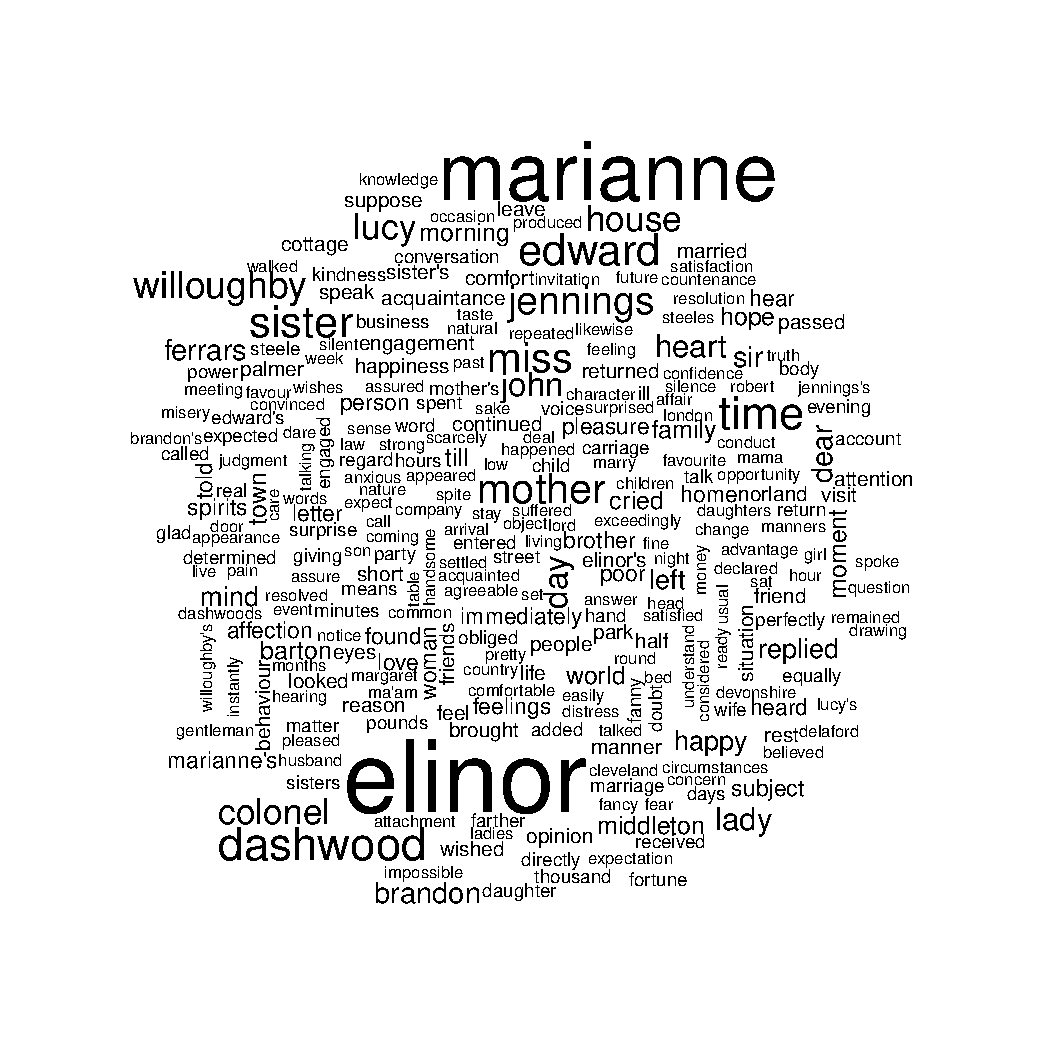
\includegraphics[width=\maxwidth]{figure/unnamed-chunk-6-1} 
\begin{kframe}\begin{alltt}
\hlcom{#make a word cloud}
\end{alltt}
\end{kframe}
\end{knitrout}


\end{document}
